\documentclass[a4paper,11pt]{article}
\usepackage{amsmath,amsthm,amsfonts,amssymb,amscd,amstext,vmargin,graphics,graphicx,tabularx,multicol} \usepackage[french]{babel}
\usepackage[utf8]{inputenc}  
\usepackage[T1]{fontenc} 
\usepackage[T1]{fontenc}
\usepackage{amsmath,amssymb}
\usepackage{pstricks-add,tikz,tkz-tab,variations}
\usepackage[autolanguage,np]{numprint} 

\setmarginsrb{1.5cm}{0.5cm}{1cm}{0.5cm}{0cm}{0cm}{0cm}{0cm} %Gauche, haut, droite, haut
\newcounter{numexo}
\newcommand{\exo}[1]{\stepcounter{numexo}\noindent{\bf Exercice~\thenumexo} : \marginpar{\hfill /#1}}
\reversemarginpar


\newcounter{enumtabi}
\newcounter{enumtaba}
\newcommand{\q}{\stepcounter{enumtabi} \theenumtabi.  }
\newcommand{\qa}{\stepcounter{enumtaba} (\alph{enumtaba}) }
\newcommand{\initq}{\setcounter{enumtabi}{0}}
\newcommand{\initqa}{\setcounter{enumtaba}{0}}

\newcommand{\be}{\begin{enumerate}}
\newcommand{\ee}{\end{enumerate}}
\newcommand{\bi}{\begin{itemize}}
\newcommand{\ei}{\end{itemize}}
\newcommand{\bp}{\begin{pspicture*}}
\newcommand{\ep}{\end{pspicture*}}
\newcommand{\bt}{\begin{tabular}}
\newcommand{\et}{\end{tabular}}
\renewcommand{\tabularxcolumn}[1]{>{\centering}m{#1}} %(colonne m{} centrée, au lieu de p par défault) 
\newcommand{\tnl}{\tabularnewline}

\newcommand{\trait}{\noindent \rule{\linewidth}{0.2mm}}
\newcommand{\hs}[1]{\hspace{#1}}
\newcommand{\vs}[1]{\vspace{#1}}

\newcommand{\N}{\mathbb{N}}
\newcommand{\Z}{\mathbb{Z}}
\newcommand{\R}{\mathbb{R}}
\newcommand{\C}{\mathbb{C}}
\newcommand{\Dcal}{\mathcal{D}}
\newcommand{\Ccal}{\mathcal{C}}
\newcommand{\mc}{\mathcal}

\newcommand{\vect}[1]{\overrightarrow{#1}}
\newcommand{\ds}{\displaystyle}
\newcommand{\eq}{\quad \Leftrightarrow \quad}
\newcommand{\vecti}{\vec{\imath}}
\newcommand{\vectj}{\vec{\jmath}}
\newcommand{\Oij}{(O;\vec{\imath}, \vec{\jmath})}
\newcommand{\OIJ}{(O;I,J)}

\newcommand{\bmul}[1]{\begin{multicols}{#1}}
\newcommand{\emul}{\end{multicols}}


\newcommand{\reponse}[1][1]{%
\multido{}{#1}{\makebox[\linewidth]{\rule[0pt]{0pt}{20pt}\dotfill}
}}

\newcommand{\titre}[5] 
% #1: titre #2: haut gauche #3: bas gauche #4: haut droite #5: bas droite
{
\noindent #2 \hfill #4 \\
#3 \hfill #5

\vspace{-1.6cm}

\begin{center}\rule{6cm}{0.5mm}\end{center}
\vspace{0.2cm}
\begin{center}{\large{\textbf{#1}}}\end{center}
\begin{center}\rule{6cm}{0.5mm}\end{center}
}



\begin{document}
\pagestyle{empty}
\titre{Contrôle : Nombres relatifs (1) et (2)}{Nom :}{Prénom :}{Classe}{Date}

\vspace*{0.5cm}

\begin{flushleft}
\begin{tabular}{|m{6cm}|m{2.5cm}|m{2.5cm}|m{2.5cm}|m{2.5cm}|}
\hline 
\textbf{Compétences} & \begin{center}
\textbf{Très bonne maîtrise}
\end{center} & \begin{center}
\textbf{Maîtrise satisfaisante}
\end{center}  & \begin{center}
\textbf{Maîtrise faible}
\end{center} & \begin{center}
\textbf{Maîtrise insuffisante}
\end{center} \\ 
\hline 
Je dois savoir ranger et comparer des nombres relatifs &  &  & &\\
\hline
Je dois savoir lire les coordonnées d'un point donné dans le plan muni d'un repère orthogonal &  &  & & \\ 
\hline
Je dois savoir calculer la somme et la différence de deux nombres relatifs de même signe &  &  &  &\\ 
\hline 
Je dois savoir  calculer avec des nombres relatifs, en combinant de façon appropriée le calcul mental, le calcul posé  &  &  &  &\\ 
\hline 
Je dois savoir déterminer la distance entre deux points   &  &  &  &\\ 
\hline   
Je dois savoir traduire en langage mathématique une situation réelle   &  &  &  &\\ 
\hline 

\end{tabular} 
\end{flushleft}

\vspace*{0.5cm}
\vspace*{0.5cm}


\exo{2} Dans cet exercice, vous justifierez vos réponses par \textbf{des calculs}.\\

\initq

\q Un sous marin qui naviguait à $-534$~m remonte à $-197$~m ; de
combien de mètres a-t-il remonté ?\\
Il redescend à $-732$~m, de combien de mètres est-il descendu ?\\

\q Les guerres puniques opposèrent Rome à Carthage.\\

\qa La première commença en $-264$ et s'acheva en $-241$ par la
victoire de Rome, combien de temps dura-t-elle ?\\
\qa Hannibal déclencha la seconde qui dura 17 ans et s'acheva en
$-201$, par la victoire du romain Scipion, en quelle année a-t-elle
commencé ?\\


\vspace*{0.5cm}

\exo{1.5}  \\

Compléter sur le sujet la pyramide ci-dessous en sachant que chaque case contient le somme des nombres contenus dans les deux cases du dessous.



\begin{center}
\includegraphics[scale=0.7]{pyramiderelatifs2.eps}
 \end{center} 


\newpage

\exo{3.5}

 \begin{pspicture*}(-7.,-2.)(10.,2.)
\psaxes[labelFontSize=\scriptstyle,xAxis=true,yAxis=false,Dx=0.2,dx=0.75,ticksize=-2pt 0,subticks=1]{->}(0,0)(-7.,-2.)(10.,2.)
\end{pspicture*} 

\initq 
\noindent \q Placer sur la droite graduée ci-dessus, les points A, B et C d'abscisses respectives 1,8 ; -1,6 et 0,2.\\
\q Calculer les distances AC et BC.\\
\q Que peut-on dire du point C ? (Justifier)\\


\exo{7}

\bmul{2}

\initq \q Lire et écrire les coordonnées des points A, B, C, D, E, F et G de la figure.\\

\q Quels sont ceux qui ont :\\
\initqa \qa une abscisse négative non nulle ? \\
 \qa une ordonnée négative non nulle ?  \\
   \qa une abscisse positive et une ordonnée négative ?

\columnbreak

\includegraphics[scale=1]{reperageplan.eps} 


\emul


\exo{6} 

\bmul{2}
Des enfants lancent 4 fléchettes sur la cible représentée ci-contre.\\
On obtient :\\
\bi
\item 5 points pour un tir dans le rouge,
\item 2,5 points pour un tir dans le vert,
\item -1,75 point pour un tir dans le bleu,
\item -8 points si on rate la cible.
\ei

\columnbreak

\begin{center}
 
\includegraphics[scale=1]{cible.eps}
 \end{center} 
\emul

Voici les résultats des 4 compétiteurs :
\bmul{2}
\noindent Anaïs : rouge, vert, vert, raté\\
David : rouge, vert, bleu, raté

\columnbreak

\noindent Eva : rouge, raté, raté, rouge\\
Sacha : vert, vert, bleu, raté

\emul

\initq
\q 
\initqa \qa\textbf{ Écrire }l'expression qui permet de calculer le score de chaque enfant, puis \textbf{calculer} ce score.\\
\qa \textbf{Ranger} ces scores par ordre croissant.\\

\q Un enfant a obtenu le score de -8,5. Quels sont ses 4 lancers ?\\



\exo{} BONUS\\

\textbf{Trouve le bon chemin pour sortir du labyrinthe parallélépipédique ci-dessous.}

\bmul{2}

Tu peux te déplacer :\\

– soit horizontalement (sur le même étage), mais tu ne peux passer d'une case à l'autre que si les deux cases ont un côté commun et si le nombre de la case où tu vas est supérieur à celui de le case d'origine.\\

– soit verticalement (d'un étage à un autre), mais tu ne peux descendre que si la case du dessous contient un nombre inférieur à la case à celle du dessus.\\

\columnbreak

\begin{center}
 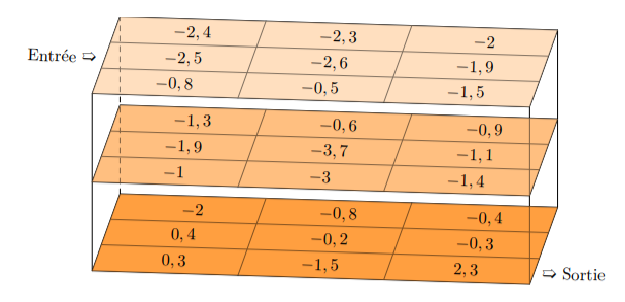
\includegraphics[scale=1]{bonus.eps}
 \end{center} 
 
 \emul

\end{document}
